\documentclass[a4paper,12pt, tikz]{scrartcl}
\usepackage{pdflscape}
\usepackage{tabularx}
\usepackage{lipsum}
\usepackage{color}
\usepackage{enumitem,amssymb, amsmath}
\usepackage{xcolor}
\usepackage{tikz}
\usepackage{tkz-euclide}

\newcommand\Vtextvisiblespace[1][.3em]{%
  \mbox{\kern.06em\vrule height.3ex}%
  \vbox{\hrule width#1}%
  \hbox{\vrule height.3ex}}
\newcommand{\checkbox}{ {\fboxsep=-.2pt\fbox{\rule{0pt}{2ex}\rule{2ex}{0pt}}}}

\newcommand{\subtablaDescrip}{ \begin{tabular}{ll}&\\ prioridad: & \Vtextvisiblespace[2em] \\ dificultad: & \Vtextvisiblespace[2em]\\&\\ \end{tabular}}

\begin{document}


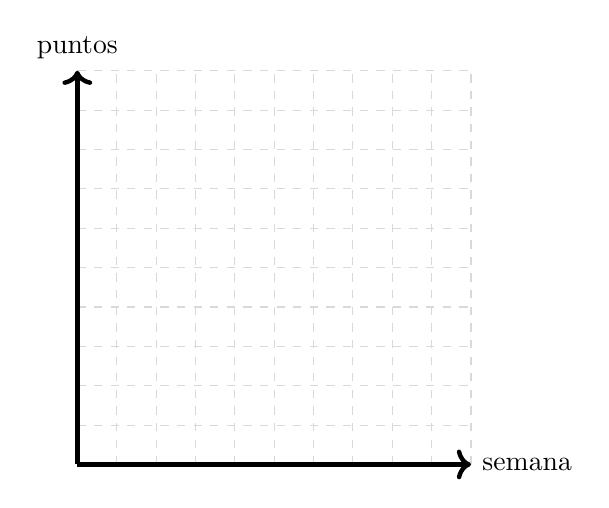
\begin{tikzpicture}[scale=0.5]
    \tkzInit[xmin=-5,xmax=5,ymin=-5,ymax=5]
    
    \draw[help lines, color=gray!30, dashed] (0,0) grid (10,10);
    \draw[->,ultra thick] (0,0)--(10,0) node[right]{semana};
    \draw[->,ultra thick] (0,0)--(0,10) node[above]{puntos};
    
    \end{tikzpicture}

    \newpage

    \section*{Semana DATE1 -- DATE2}
    \thispagestyle{empty}
    \noindent
    \begin{tabularx}{\linewidth}{|X|c c|}
        \hline
      \textbf{Tarea} & \textbf{descripción} & \textbf{proceso}\\
      \hline
       1.\vspace{4ex} &      \subtablaDescrip     & $\square\square\square\square\square$ \\
      \hline
      2.\vspace{4ex} &      \subtablaDescrip     & $\square\square\square\square\square$ \\
      \hline
      3.\vspace{4ex} &      \subtablaDescrip     & $\square\square\square\square\square$ \\
      \hline
      4.\vspace{4ex} &      \subtablaDescrip     & $\square\square\square\square\square$ \\
      \hline
      5.\vspace{4ex} &      \subtablaDescrip     & $\square\square\square\square\square$ \\
      \hline
      6.\vspace{4ex} &      \subtablaDescrip     & $\square\square\square\square\square$ \\
      \hline
      7.\vspace{4ex} &      \subtablaDescrip     & $\square\square\square\square\square$ \\
      \hline
      8.\vspace{4ex} &      \subtablaDescrip     & $\square\square\square\square\square$ \\
      \hline
      9.\vspace{4ex} &      \subtablaDescrip     & $\square\square\square\square\square$ \\
      \hline
      10.\vspace{4ex} &      \subtablaDescrip     & $\square\square\square\square\square$ \\
      \hline
    \end{tabularx}

    \newpage
 


\begin{center}
\begin{tabular}{ll}
    \textbf{Facilidades} & \textbf{Dificultades} \\
  \fcolorbox{black!50!black}{white}{
    \begin{tabular}{c}
    \phantom{Lorem ipsum dolor sit amet, consectetur}\\
    \phantom{Lorem ipsum dolor sit amet, consectetur}\\
    \end{tabular}

  } &
  \fcolorbox{black!50!black}{white}{
    \begin{tabular}{c}
        \phantom{Lorem ipsum dolor sit amet, consectetur}\\
        \phantom{Lorem ipsum dolor sit amet, consectetur}\\
        \end{tabular}
  } \\
\end{tabular}
\end{center}

\begin{center}
\textbf{Reflexiones}\\ \vspace{3ex}
\fcolorbox{black!50!black}{white}{
    \begin{tabular}{l}
    \phantom{Lorem ipsum dolor sit amet, consectetur Lorem  Lorem ipsum dolor sit amet, consectetur}\\
    \phantom{Lorem ipsum dolor sit amet, consectetur}\\
    \phantom{Lorem ipsum dolor sit amet, consectetur}\\
    \phantom{Lorem ipsum dolor sit amet, consectetur}\\
    \phantom{Lorem ipsum dolor sit amet, consectetur}\\
    \phantom{Lorem ipsum dolor sit amet, consectetur}\\
    \phantom{Lorem ipsum dolor sit amet, consectetur}\\
    \phantom{Lorem ipsum dolor sit amet, consectetur}\\
    \phantom{Lorem ipsum dolor sit amet, consectetur}\\
    \end{tabular}
  }
\end{center}
\vspace{5ex}

\begin{center}
    \textbf{Notas}\\ \vspace{3ex}
    \fcolorbox{black!50!black}{white}{
        \begin{tabular}{l}
        \phantom{Lorem ipsum dolor sit amet, consectetur Lorem  Lorem ipsum dolor sit amet, consectetur}\\
        \phantom{Lorem ipsum dolor sit amet, consectetur}\\
        \phantom{Lorem ipsum dolor sit amet, consectetur}\\
        \phantom{Lorem ipsum dolor sit amet, consectetur}\\
        \phantom{Lorem ipsum dolor sit amet, consectetur}\\
        \phantom{Lorem ipsum dolor sit amet, consectetur}\\
        \phantom{Lorem ipsum dolor sit amet, consectetur}\\
        \phantom{Lorem ipsum dolor sit amet, consectetur}\\
        \phantom{Lorem ipsum dolor sit amet, consectetur}\\
        \end{tabular}
      }
    \end{center}

\vspace{5ex}
Resultado semana: \Vtextvisiblespace[2em]

\end{document}